% L9c gradient descent schematic: a loss with a local minimum theta_2 and a
% lower minimum theta_1. Gradient descent started at theta_3 goes downhill to
% theta_2; started at theta_0 it goes downhill to theta_1.
%
% Redrawn on October 9, 2026 after the Fall 2025 schematic, which set the
% labels with a capital theta and no subscripts. Labels follow the lecture:
% lowercase theta with subscripts and the gradient written \nabla_{\theta}.
%
% The curve is four cubic Bezier segments with horizontal handles at each
% extremum, so the local minimum (1.40, 2.30), the hump (2.80, 2.95), and the
% lower minimum (5.60, 0.65) sit exactly at those points. The start points and
% unit tangents were computed from the same control points:
%   theta_3: segment 1 at t = 0.12 -> (0.353, 4.828), tangent (0.0951, -0.9955)
%   theta_0: segment 4 at t = 0.72 -> (8.026, 2.233), tangent (0.6638,  0.7479)
% Each gradient arrow follows the tangent direction and points downhill.
%
% Math uses the standard TeX fonts (no unicode-math), so \theta renders as the
% same plain theta the notebook's math shows.
%
% The notebook SVG carries a dark palette added by theme_svg.py; keep new
% colors in that script's mapping when changing the palette here.
\documentclass[tikz,border=4pt]{standalone}
\usepackage[no-math]{fontspec}
\IfFontExistsTF{Arial}{\setsansfont{Arial}}{\setsansfont{TeX Gyre Heros}}
\renewcommand{\familydefault}{\sfdefault}
\usepackage{amsmath,amssymb}
\usetikzlibrary{arrows.meta,calc}

% Ink matches the L7c schematic; the four point colors are the 2025 figure's.
\definecolor{vnink}{HTML}{202124}
\definecolor{gdblue}{HTML}{0091FF}
\definecolor{gdgreen}{HTML}{6EB43F}
\definecolor{gdred}{HTML}{E02020}
\definecolor{gdgray}{HTML}{6D7278}

\begin{document}
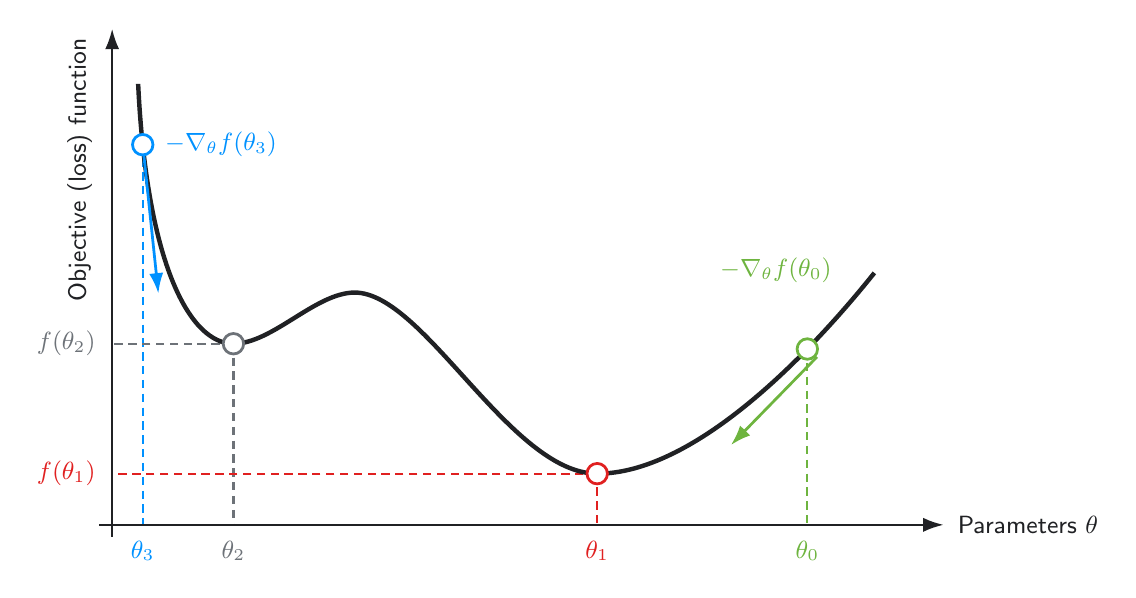
\begin{tikzpicture}[x=1.1cm, y=1cm, font=\sffamily\small, text=vnink,
    axis/.style={draw=vnink, line width=0.8pt, -{Latex[length=2.6mm, width=1.8mm]}},
    loss/.style={draw=vnink, line width=1.6pt},
    drop/.style={line width=0.8pt, dash pattern=on 3pt off 2pt},
    grad/.style={line width=1.0pt, -{Latex[length=2.6mm, width=1.8mm]}},
    pt/.style={circle, fill=white, line width=1.0pt, inner sep=0pt, minimum size=2.6mm},
  ]
  % start points and minima
  \coordinate (t3) at (0.353, 4.828);
  \coordinate (t2) at (1.40, 2.30);
  \coordinate (t1) at (5.60, 0.65);
  \coordinate (t0) at (8.026, 2.233);

  % dashed guides to the axes, drawn first so everything else sits on top
  \draw[drop, gdblue] (t3) -- (t3 |- 0,0);
  \draw[drop, gdgray] (t2) -- (t2 |- 0,0);
  \draw[drop, gdgray] (t2) -- (0, 2.30);
  \draw[drop, gdred] (t1) -- (t1 |- 0,0);
  \draw[drop, gdred] (t1) -- (0, 0.65);
  \draw[drop, gdgreen] (t0) -- (t0 |- 0,0);

  % axes
  \draw[axis] (-0.15, 0) -- (9.6, 0);
  \draw[axis] (0, -0.15) -- (0, 6.3);
  \node[anchor=west] at (9.65, 0) {Parameters $\theta$};
  \node[rotate=90, anchor=south east] at (-0.12, 6.3) {Objective (loss) function};

  % loss curve
  \draw[loss] (0.30, 5.60) .. controls (0.40, 3.30) and (0.90, 2.30) .. (1.40, 2.30)
    .. controls (1.85, 2.30) and (2.35, 2.95) .. (2.80, 2.95)
    .. controls (3.60, 2.95) and (4.60, 0.65) .. (5.60, 0.65)
    .. controls (6.70, 0.65) and (8.00, 2.10) .. (8.80, 3.20);

  % negative gradients: start at the point and run downhill along the tangent
  % (1.9 and 1.5 units). The green arrow is shifted 0.15 units off the curve
  % along the normal (0.7479, -0.6638) so the two lines do not overlap.
  \draw[grad, gdblue] (t3) -- ($(t3) + (0.1807, -1.8915)$);
  \draw[grad, gdgreen] ($(t0) + (0.1122, -0.0996)$) -- ($(t0) + (0.1122, -0.0996) + (-0.9957, -1.1219)$);
  \node[anchor=west, text=gdblue] at (0.50, 4.83) {$-\nabla_{\theta} f(\theta_{3})$};
  \node[anchor=south east, text=gdgreen] at (8.42, 2.95) {$-\nabla_{\theta} f(\theta_{0})$};

  % axis labels for the four points
  \node[anchor=north, text=gdblue] at (t3 |- 0,-0.08) {$\theta_{3}$};
  \node[anchor=north, text=gdgray] at (t2 |- 0,-0.08) {$\theta_{2}$};
  \node[anchor=north, text=gdred] at (t1 |- 0,-0.08) {$\theta_{1}$};
  \node[anchor=north, text=gdgreen] at (t0 |- 0,-0.08) {$\theta_{0}$};
  \node[anchor=east, text=gdgray] at (-0.08, 2.30) {$f(\theta_{2})$};
  \node[anchor=east, text=gdred] at (-0.08, 0.65) {$f(\theta_{1})$};

  % open markers last
  \node[pt, draw=gdblue] at (t3) {};
  \node[pt, draw=gdgray] at (t2) {};
  \node[pt, draw=gdred] at (t1) {};
  \node[pt, draw=gdgreen] at (t0) {};
\end{tikzpicture}
\end{document}
